





\begin{abstract}
	By recursively nesting sums and products, probabilistic circuits (PCs) have emerged in recent years as an attractive class of generative models as they enjoy, for instance, polytime marginalization of random variables.
	However, as these PCs form monotone functions, specifically the parameters are constrained to positive real values, their expressive power is limited.
	Drawing inspiration quantum information theory we introduce \textit{positive unitary circuits} (\puncs),
	which generalize circuit evaluations over positive real-valued probabilities to circuit evaluation over positive semidefinite matrices.
	A key feature of \puncs is that they form normalized probability distributions by construction, which avoids the computation of a spurious normalization constant.
	Motivated by noisy quantum systems we generalize \puncs to \noisepuncs, which can be interpreted as deep mixtures of \puncs.
	Lastly, we provide an efficient parametrization of \puncs that enables us to perform parameter learning on hardware accelerators using standard and unconstrained gradient-based optimization.
\end{abstract}




\section{Introduction}


Probabilistic circuits (PCs)~\citep{darwiche2003differential,poon2011sum} belong to an unusual class of probabilistic models: they are highly expressive but at the same time also tractable.
For instance, so-called decomposable probabilistic circuits~\citep{darwiche2001decomposable} allow for the computation of marginals in time polynomial in the size of the circuit.
\citet{zhang2020relationship} noted that it is exactly this restriction to positive values that limits the expressive efficiency (or succinctness) of PCs~\citep{martens2014expressive,decolnet2021compilation}. In particular, the positivity constraint on the set of elements that PCs operate on prevents them from modelling negative correlations between variables.
Circuits that are incapable of modelling negative correlations, \ie circuits that can only combine probabilities in an additive fashion, are also called monotone circuits~\citep{shpilka2010arithmetic}.
This restricted expressiveness can be combatted by the use of so-called \textit{non-monotone} circuits, where subtractions are allowed as a third operation (besides sums and products). Interestingly, \citet{valiant1979negation} showed that a mere single subtraction can render non-monotone circuits exponentially more expressive than monotone circuits a result that has recently been refined for decomposable circuits~\citep{loconte2024sum}.

As shown in \citep{harviainen2023inference,agarwalprobabilistic}, non-monotone circuits do, however, introduce an important complication: if non-monotone circuits are not designed carefully, verifying whether a circuit encodes a valid probability distribution or not is an NP-hard problem. This does also render learning the parameters of a circuit practically infeasible.

Using the concept of \textit{positive operator valued measures} from quantum information theory, which encode random event as positive semidefinite matrices we are able to construct non-monotone circuits that nonetheless encode proper (normalized) probability distributions by construction.
Our work falls into a line of recent works presented in the circuit literature ~\citep{sladek2023encoding,loconte2024subtractive,wangrelationship,loconte2024sum}. However, our work is the first that establishes this deep connection between concepts in quantum information theory and tractable probabilistic models. We make three concrete contributions
\begin{enumerate*}
	\item We generalize probabilistic circuits over scalars to operator-valued circuits and introduce \puncs (Section~\ref{sec:puncs}).
	\item We use the concept of noise in quantum information theory to construct deep operator mixture circuits, dubbed \noisepuncs (Section~\ref{sec:noisecircuits}).
	\item We provide an efficient parametrization such that the constructed probability distributions using \puncs are normalized by construction (Section~\ref{sec:efficient_param}).
\end{enumerate*}






%%%%%%%%%%%%%%%%%%%%%%%%%%%%%%%%%%%%%%%%%%%%%%%%%%%%%%%%%%%%%%%%%%%%%%%%%%%%%%%%%
%%%%%%%%%%%%%%%%%%%%%%%%%%%%%%%%%%%%%%%%%%%%%%%%%%%%%%%%%%%%%%%%%%%%%%%%%%%%%%%%%
%%%%%%%%%%%%%%%%%%%%%%%%%%%%%%%%%%%%%%%%%%%%%%%%%%%%%%%%%%%%%%%%%%%%%%%%%%%%

\section{A Primer on Quantum Information Theory}
\label{sec:qit}


A widely used and elegant framework to describe measurements of quantum systems is the so-called \textit{positive operator-valued measure} (POVM) formalism. While POVMs have physical interpretations in terms of quantum information and quantum statistics, we will only be interested in their mathematical prperties as we use them to show that  circuits (defined in Section~\ref{sec:puncs}) form valid probability distributions.
We refer the reader to \citep{nielsen2001quantum} for an in-depth exposition on the topic, as well as quantum computing and quantum information theory in general.
\begin{definition}[Positive Semidefinite]
	An $\numbond {\times} \numbond$ Hermitian matrix $H$ is called positive semidefinite (PSD) if and only if $\forall \xvars {\in}  \mathbb {C} ^{\numbond}: \xvars^{*} H \xvars {\geq} 0$, where $\xvars^{*}$ denotes the conjugate transpose and $\mathbb {C}^{\numbond}$ the $\numbond$-dimensional space of complex numbers.
\end{definition}
\begin{definition}[{POVM~\citep[Page 90]{nielsen2001quantum}}]
	\label{def:povm}
	A positive operator-valued measure
	% with a finite number of elements acting on a finite-dimensional Hilbert space $\mathcal{H}$,
	is a set of PSD  matrices $\{E(i)\}_{i=0}^{\numevents-1}$ ($I$ being the number of possible measurement outcomes) that sum to the identity:
	\begin{talign}
		\sum_{i=0}^{\numevents-1} E(i) = \mathbb{1},
		\label{eq:povm_normalized}
	\end{talign}
\end{definition}
Before defining the probability of a specific $i$ occurring, we need the notion of a density matrix~\citep{neumann1927wahrscheinlich}:
\begin{definition}[{Density Matrix~\citep[Page 102]{nielsen2001quantum}}]
	\label{def:density_matrix}
	A density matrix $\rho$ is a PSD matrix of trace one, \ie $\Tr [\rho]=1$.
\end{definition}
\begin{definition}[{Event Probability~\citep[Page 102]{nielsen2001quantum}}]
	\label{def:eventprob}
	Let $\rho$ be a density matrix and let $i$ denote an event with $E(i)$ being the corresponding element from the POVM. The probability of the event $i$ happening, \ie measuring the outcome $i$, is given by
	\begin{talign}
		p(i) = \Tr [ \rho E(i)]
		\label{eq:povm_prob}
	\end{talign}
\end{definition}




%%%%%%%%%%%%%%%%%%%%%%%%%%%%%%%%%%%%%%%%%%%%%%%%%%%%%%%%%%%%%%%%%%%%%%%%%%%%%%%%%
%%%%%%%%%%%%%%%%%%%%%%%%%%%%%%%%%%%%%%%%%%%%%%%%%%%%%%%%%%%%%%%%%%%%%%%%%%%%%%%%%
%%%%%%%%%%%%%%%%%%%%%%%%%%%%%%%%%%%%%%%%%%%%%%%%%%%%%%%%%%%%%%%%%%%%%%%%%%%%




\begin{restatable}{proposition}{proppovmprob}
	\label{prop:povmprob}
	The expression in Equation~\ref{eq:povm_prob} defines a valid probability distribution.
\end{restatable}

\begin{proof}
	While this is a well-known result we were not able to identify a concise proof in the literature. We therefore provide one in Appendix~\ref{sec:proof:prop:povmprob}.
\end{proof}



\todo{talk about Loewner order}


\citep[Corollary 4.2]{baksalary1989some}






















\section{Positive Unitary Circuits}
\label{sec:puncs}

\begin{figure}[t]

	\centering
	\begin{minipage}{0.45\textwidth}
	\centering
	\resizebox{0.9\columnwidth}{!}{
		\tikzset{point/.style={circle,inner sep=0pt,minimum size=3pt,fill=red}}
	\centering

	\begin{tikzpicture}

		\sumnode[line width=\midlinewidth]{v11};
		\sumnode[line width=\midlinewidth, right=\halfdist of v11]{v12};
		\sumnode[line width=\midlinewidth, right=\halfdist of v12]{v13};
		\sumnode[line width=\midlinewidth, right=\middist of v13]{v21};
		\sumnode[line width=\midlinewidth, right=\halfdist of v21]{v22};
		\sumnode[line width=\midlinewidth, right=\halfdist of v22]{v23};

		\prodnode[line width=\midlinewidth, above=\smalldist of v13]{p121};
		\prodnode[line width=\midlinewidth, right=\halfdist of p121]{p122};
		\prodnode[line width=\midlinewidth, right=\halfdist of p122]{p12k};

		\sumnode[line width=\midlinewidth, above=\smalldist of p121]{s121};
		\sumnode[line width=\midlinewidth, above=\smalldist of p122]{s122};
		\sumnode[line width=\midlinewidth, above=\smalldist of p12k]{s12k};





		% edges
		\edge[line width=\midlinewidth,dashed] {p121} {v11, v21};
		\edge[line width=\midlinewidth,dashed] {p122} {v12, v22};
		\edge[line width=\midlinewidth,dashed] {p12k} {v13, v23};

		\edge[line width=\midlinewidth,left] {s121, s122, s12k} {p121, p122, p12k};

		%%%%% V3 and V4
		\sumnode[line width=\midlinewidth, right=\middist of v23]{v31};
		\sumnode[line width=\midlinewidth, right=\halfdist of v31]{v32};
		\sumnode[line width=\midlinewidth, right=\halfdist of v32]{v33};
		\sumnode[line width=\midlinewidth, right=\smalldist of v33]{v41};
		\sumnode[line width=\midlinewidth, right=\halfdist of v41]{v42};
		\sumnode[line width=\midlinewidth, right=\halfdist of v42]{v43};

		\prodnode[line width=\midlinewidth, above=\smalldist of v33]{p341};
		\prodnode[line width=\midlinewidth, right=\halfdist of p341]{p342};
		\prodnode[line width=\midlinewidth, right=\halfdist of p342]{p34k};

		\sumnode[line width=\midlinewidth, above=\smalldist of p341]{s341};
		\sumnode[line width=\midlinewidth, above=\smalldist of p342]{s342};
		\sumnode[line width=\midlinewidth, above=\smalldist of p34k]{s34k};


		% edges
		\edge[line width=\midlinewidth,dashed] {p341} {v31, v41};
		\edge[line width=\midlinewidth,dashed] {p342} {v32, v42};
		\edge[line width=\midlinewidth,dashed] {p34k} {v33, v43};

		\edge[line width=\midlinewidth,left] {s341, s342, s34k} {p341, p342, p34k};


		%%%% final root
		\prodnode[line width=\midlinewidth, above=95pt of v23]{p12341};
		\prodnode[line width=\midlinewidth, right=\halfdist of p12341]{p12342};
		\prodnode[line width=\midlinewidth, right=\halfdist of p12342]{p1234k};

		\sumnode[line width=\midlinewidth, above=\smalldist of p12342]{s12341};

		\edge[line width=\midlinewidth,dashed] {p12341} {s121, s341};
		\edge[line width=\midlinewidth,dashed] {p12342} {s122, s342};
		\edge[line width=\midlinewidth,dashed] {p1234k} {s12k, s34k};

		\edge[line width=\midlinewidth,left] {s12341} {p12341, p12342, p1234k};

		%%%%%%%%%%%%%%%%%%%%%%%%%%%%
		% inputs

		\varnode[line width=\midlinewidth, below left=\smalldist and 0.5\halfdist of v12]{var11}{$x^0_0$};
		\varnode[line width=\midlinewidth, below right=\smalldist and 0.5\halfdist of v12]{var12}{$x^1_0$};

		\edge[line width=\midlinewidth,left] {var11} {v11, v12, v13};
		\edge[line width=\midlinewidth,left] {var12} {v11, v12, v13};

		\varnode[line width=\midlinewidth, below left=\smalldist and 0.5\halfdist of v22]{var21}{$x^0_1$};
		\varnode[line width=\midlinewidth, below right=\smalldist and 0.5\halfdist of v22]{var22}{$x^1_1$};

		\edge[line width=\midlinewidth,left] {var21} {v21, v22, v23};
		\edge[line width=\midlinewidth,left] {var22} {v21, v22, v23};

		\varnode[line width=\midlinewidth, below left=\smalldist and 0.5\halfdist of v32]{var31}{$x^0_2$};
		\varnode[line width=\midlinewidth, below right=\smalldist and 0.5\halfdist of v32]{var32}{$x^1_2$};

		\edge[line width=\midlinewidth,left] {var32} {v31, v32, v33};
		\edge[line width=\midlinewidth,left] {var31} {v31, v32, v33};


		\varnode[line width=\midlinewidth, below left=\smalldist and 0.5\halfdist of v42]{var41}{$x^0_3$};
		\varnode[line width=\midlinewidth, below right=\smalldist and 0.5\halfdist of v42]{var42}{$x^1_3$};

		\edge[line width=\midlinewidth,left] {var42} {v41, v42, v43};
		\edge[line width=\midlinewidth,left] {var41} {v41, v42, v43};



	\end{tikzpicture}
	}
\end{minipage}
\hfill
\begin{minipage}{0.45\textwidth}
	\centering
	\begin{tikzpicture}[
			dot/.style = {circle, draw, fill, minimum size=4pt, inner sep=0pt},
			level distance=1.25cm,
			level 1/.style={sibling distance=3cm},
			level 2/.style={sibling distance=1.5cm},
			scale=1
		]

		\node[dot] (00) {}
		child {node[dot] (10) {}
				child {node[dot] (20) {}}
				child {node[dot] (21) {}}
			}
		child {node[dot] (11) {}
				child {node[dot] (22) {}}
				child {node[dot] (23) {}}
			};

		\node[below= 0.1 of 20, inner sep=0pt] (X1) {\tiny{$X_0$}};
		\node[below= 0.1 of 21, inner sep=0pt] (x2) {\tiny{$X_1$}};
		\node[below= 0.1 of 22, inner sep=0pt] (x3) {\tiny{$X_2$}};
		\node[below= 0.1 of 23, inner sep=0pt] (x4) {\tiny{$X_3$}};
	\end{tikzpicture}
\end{minipage}

	\caption{
		Partition circuit over four binary variables $x_i$ with $i \in \{0,1,2,3\}$, which are given as inputs to the circuit. The internal nodes of the partition circuit correspond the computation units.}
	\label{fig:circuit}
\end{figure}


A popular subclass of probabilistic circuits are so-called structured decomposable  probabilistic circuits~\citep{darwiche2011sdd} that are also smooth~\citep{darwiche2001tractable}. The advantage of this circuit subclass is that they can be implemented in a rather straightforward fashion on modern AI accelerators, as demonstrated by \citet{peharz2019random,peharz2020einsum}.
\todo{cite LSE paper}
\citet{zuidberg2024probabilistic} introduced an abstraction for these smooth structured decomposable circuit dubbed \textit{partition circuits}.
We give such a circuit in Figure~\ref{fig:circuit}.


\todo{cite lse paper}
\begin{definition}[Partition Circuit~\citep{LSE}]
	\label{def:partition_circuit}
	A partition circuit over a set of variables is a parametrized computation graph taking the form of a binary tree. The partition circuit consists of two kinds of computation units:
	\textit{leaf} and \textit{internal} units, as well as a single \textit{root}.
	Units at the same distance from the root form a layer.
	Furthermore, let $\circuit_k$ denote the root unit or an internal unit. The unit $\circuit_k$ then receives its inputs from two units in the previous layer, which we denote by $\circuit_{k_l}$ and $\circuit_{k_r}$. Each computation unit is input to exactly one other unit, except the root unit, which is the input to no other unit.
\end{definition}

\subsection{Operator Circuits}

Using the concept of partition circuits we now generalize the probabilistic circuits to (unnormalized) positive operator circuits. Positive operator circuits can be thought of as generalizing circuit evaluations with probabilities to circuit evaluations with PSD matrices. Note, in the definition below we use $\Ocircuit_k$ instead of $\circuit_k$ to make this generalization explicit.
\begin{definition}[Operator Circuit]
	\label{def:poc}
	Let   $\xvars{=}\{\xvar_0,\dots ,\xvar_{\numvar{-}1}  \}$ be a set of $M$ categorical variables with domains of size $\samplespacesize$.
	We define an operator circuit as a partition circuit whose computation units take the following functional form:
	\begin{align}
		 & {\Ocircuit}_k(\xvars_k){=}
		\begin{cases}
			A_{k} \times  e_{\xvar_k} \otimes  e^*_{\xvar_k} \times A_{k}^*,
			 & \text{if $k$ is leaf}
			\\
			\bilinear_k \Bigl(\Ocircuit_{k_l}(\xvars_{k_l}), \Ocircuit_{k_l}(\xvars_{k_l}) \Bigr)
			 & \text{else}
		\end{cases}
		\label{eq:poc:def}
	\end{align}
	Here we use the symbol $\otimes$ to denote the Kronecker product.
	Furthermore, $\{e_{\xvar_k} \}_{n=0}^{\samplespacesize-1}$ is a set of $\samplespacesize$-dimensinoal orthonormal basis vectors associating each of the $\samplespacesize$ possible values for $\xvar_k$ to a specific basis vector. The functions $\bilinear_k(\cdot, \cdot)$ denote bilinear forms.
\end{definition}


\begin{definition}
	We call an operator circuit \textit{positive} if we have that the bilinear forms $\bilinear_k$ are such that
	\begin{align}
		\bilinear_k \Bigl(\Ocircuit_{k_l}(\xvars_{k_l}), \Ocircuit_{k_l}(\xvars_{k_l}) \Bigr) \quad \text{is a PSD matrix}
		\label{def:eq:bilinear_psd}
	\end{align}
	if $\Ocircuit_{k_l}(\xvars_{k_l})$ and $\Ocircuit_{k_l}(\xvars_{k_l})$ are PSD.
\end{definition}



\begin{restatable}{proposition}{proppocpsd}
	\label{prop:pocpsd}
	Positive operator circuits are PSD.
\end{restatable}

\begin{proof}
	See Appendix~\ref{sec:proof:prop:pocpsd}.
\end{proof}






\subsection{Constructing a Probability Distribution}


In Section~\ref{sec:qit} we saw that we can construct a probability distribution using a density matrix $\rho$ and a positive operator-valued measure, with the latter being a set of PSD matrices (\cf Definition~\ref{def:povm}) that sum to the unit matrix. Using a positive operator circuit $\Ocircuit(\xvars)$ we indeed have a set of PSD matrices. Namely, on for each instantiation of the $\xvars$ variables. We now introduce \textit{positive unit preserving operator circuits} for which also the summation to the unit matrix holds.

\begin{definition}
	\label{def:bilinear_unitpreserving}
	We call a positive operator circuit \textit{unit preserving} if we have that the bilinear forms $\bilinear_k$ are such that
	\begin{align}
		\bilinear_k(\mathbb{1}_{k_l}, \mathbb{1}_{k_r})= \mathbb{1}_k,
		\label{def:eq:bilinear_unitpreserving}
	\end{align}
	where $\mathbb{1}_{k}$, $\mathbb{1}_{k_l}$ , and $\mathbb{1}_{k_r}$  denote unit matrices of appropriate size, and if $A_{k}A_{k}^{*}= \mathbb{1}_{k}$ in the leaves. That is, the $A_{k}$ are semi-unitary matrices.
\end{definition}
We will also refer to positive unit preserving operator circuits as positive unitary circuits, or \puncs.


\begin{restatable}{proposition}{proppuncPOVM}
	\label{prop:puncPOVM}
	Let $\Xvars$ denote a set of random variables with sample space $\Omega(\Xvars)$.
	Then the set $\{ \punccircuit(\xvars)\}_{\xvars \in \Omega(\Xvars)}$ of positive unitary circuis forms a POVM.
\end{restatable}

\begin{proof}
	See Appendix~\ref{sec:proof:prop:puncPOVM}
\end{proof}




\begin{restatable}{theorem}{theopuncprobdist}
	\label{theo:puncprobdist}
	Let $\rho$ be a density matrix and $\punccircuit(\xvars)$ a positive unitary circuit. The function
	\begin{align}
		p_\Xvars(\xvars) = \Tr [\punccircuit(\xvars) \rho]
		\label{eq:theo:prob_operator}
	\end{align}
	is a proper probability distribution over the random variables $\Xvars$ with sample space $\Omega(\Xvars)$.
\end{restatable}

\begin{proof}
	This follows from Proposition~\ref{prop:povmprob} and Proposition~\ref{prop:puncPOVM}
\end{proof}





\section{Quantum Noise and Circuits}
\label{sec:noisecircuits}

\subsection{Sub-Complete Probability Distributions}

An important concept in quantum information theory that generalizes the standard POVM (\cf Definition~\ref{def:povm}) is the so-called noisy POVM, which enables for instance modelling imperfect measurement devices. In the context of machine learning this might be an improperly labeled data point of an error in the detector, \eg a pixel flip in the camera that took a picture.
\begin{definition}
	\label{def:noisypovm}
	A noisy positive operator-valued measure
	is a set of PSD  matrices $\{E(i)\}_{i=0}^{I-1}$ ($\numevents$ being the number of possible measurement outcomes) such that:
	\begin{talign}
		\sum_{i=0}^{V-1} E(i) = \subcompletemeasrure < \mathbb{1},
	\end{talign}
	where the inequality sign is interpreted using the Loewner ordering of PSD matrices,
	\ie $\subcompletemeasrure < \mathbb{1} \Leftrightarrow\mathbb{1}-\subcompletemeasrure$ is PSD.
\end{definition}

\begin{definition}[Sub-complete Probability Distribution]
	Let $\Xvars$ be a set of random variables with sample space $\Omega(\Xvars)$. We call a probability distribution \textit{sub-complete} if $\forall \xvars \in \Omega(\Xvars): p(\xvars)\geq 0$ and if $\sum{\xvars \in \Omega(\Xvars)} p(\xvars)\leq 1$. We call a probability distribution \textit{striclty sub-complete} if the latter inequality holds strictly and \textit{complete} if equality holds.
\end{definition}




\begin{restatable}{proposition}{propnoisypovmdist}
	\label{prop:noisypovmdist}
	Noisy POVMs induce a sub-complete probability distributions.
\end{restatable}


\begin{proof}
	See Appendix \ref{prop:noisypovmdist}
\end{proof}



To construct sub-complete probability distributions using operator circuits we now introduce \textit{noisy positive unit preserving operator circuits} or \noisepuncs.

\begin{definition}
	\label{def:noisepunc}
	A \noisepunc $\Qcircuit(\xvars)$ is of the form
	\begin{align}
		\Qcircuit(\xvars)= \qcircuit(\xvars) \punccircuit(\xvars),
	\end{align}
	where $\punccircuit(\xvars)$ is a positive unit preserving operator circuit and $\qcircuit(\xvars)$ is real-valued and belongs to the  $[0,1]$ interval for every $\xvars$.
\end{definition}



\begin{restatable}{proposition}{propnoisepunddist}
	\label{prop:noisepunddist}
	\noisepuncs induce sub-complete probability distributions.
\end{restatable}

\begin{proof}
	See Appendix \ref{sec:proof:prop:noisepunddist}
\end{proof}




\subsection{Noise Variables}


All of this is a bit unnerving. How is it possible that we have probabilistic events $\xvars\in \Omega(\Xvars)$ that violate the second of Kolmogorov's probability axioms (by having sub-complete distributions)? The resolution to this problem lies in interpreting sub-complete distributions as joint distributions not only over the set of variables $\Xvars$ but an extra set of variables $\Yvars$ representing extra noise~\citep{wiseman2009quantum}
\begin{align}
	\pi_{\Xvars}(\xvars) = p_{\Xvars \Yvars}(\xvars, \yvars),
\end{align}
for which we indeed have
\begin{talign}
	\sum_{\xvars\in \Omega(\Xvars)} \sum_{\yvars\in \Omega(\Yvars)}  p_{\Xvars \Yvars}(\xvars, \yvars) =1.
\end{talign}
The problem with the random variables $\Yvars$ is that they are not accessible to the observer. In the sense that they are observable in principle but in practice not, \eg a defect in a sensor.\footnote{Note these practically unobservable variables should not be confused with the concept of (local) hidden variables, which lead to violations of Bell's inequality.}
However, the probability we are actually interested in is the one for $\Xvars$ given $\Yvars$
\begin{align}
	p_{\Xvars|\Yvars}(\xvars\mid \yvars )
	 & =
	\nicefrac{
	p_{\Xvars \Yvars}(\xvars,  \yvars )
	}
	{
	\sum_{\xvars\in \Omega(\Xvars)}p_{\Xvars \Yvars}(\xvars, \yvars )
	}
	\nonumber
	\\
	 & = \nicefrac{\pi_{\Xvars}(\xvars)}{\sum_{\xvars\in \Omega(\Xvars)}  \pi_{\Xvars}(\xvars)}
\end{align}
The question now became whether we can choose $\qcircuit(\xvars)$ such that the summation in the denominator is tractable, \ie can be performed in time polynomial in the number of random variables $\Xvars$.




\subsection{Soft Counting Circuits}

\todo{use probabislitc circuits instead of soft counting seems to work better}

In the probabilistic circuit literature in has been shown that the product of two circuits is representable as a single circuit within polytime and polyspace if the two circuits are compatible~\citep{khosravi2019tractable,vergari2021compositional}. Importantly, this single circuit then allows for summing out the variables $\xvars$.
We will now show that this also holds when the $\qcircuit(\xvars)$ is a circuit and $\punccircuit(\xvars)$ is a \punc, and both share the same partition tree. To this end we also introduce a new circuit type that satisfies the $0\leq \qcircuit(\xvars)\leq 1$ constraint imposed in Definition~\ref{def:noisepunc}.



\begin{definition}[Soft Counting Circuit]
	\label{def:lpc}
	Let   $\xvars{=}\{\xvar_0,\dots ,\xvar_{\numvar{-}1}  \}$ be a set of $\numvar$ categorical variables with domains of size $\samplespacesize$.
	We define an operator circuit as a partition circuit whose computation units take the following functional form:
	\begin{align}
		{\qcircuit}_k(\xvars_k)=
		\begin{cases}
			W_k \times  \text{one\_hot}(\xvar_k),
			 & \text{if $k$ leaf}
			\\
			W_k \times \Bigl( \qcircuit_{k_l}(\xvars_{k_l}) \odot  \qcircuit_{k_r} (\xvars_{k_r}) \Bigr)
			 & \text{else}.
		\end{cases}
		\nonumber
	\end{align}
	Here we use the symbols $\times$ and $\odot$ to denote the matrix product and Hadamard product, respectively.
	In the leaves we have $W_k\in \mathbb{R}_{\geq 0}^{\numcomponents \times \samplespacesize}$ with $\numcomponents$ being a positive integer determining the capacity of the circuit. We also require the entries of $W_k$ in the leaves to be upper bounded by $1$.
	For the $W_k$ in the internal units and the root unit we require their entries to be positive reals and that they are row-normalized. That is, $\forall k,i: \sum_j W_{kij}=1$, where the $i$ and $j$ indices index the matrix. For internal units we have $W_k\in \mathbb{R}_{\geq 0}^{\numcomponents \times \numcomponents}$ and for the root we have $W_{root} \in \mathbb{R}_{\geq 0}^{1 \times \numcomponents}$.
\end{definition}


For the sake of simplicity we have chosen here a canonical polyadic form~\citep{carroll1970analysis} for the internal units by using a Hadamard product to decompose variable sets. We refer the reader to ~\citep{loconte2024relationship} for discussions on alternative decomposition strategies.





\begin{restatable}{proposition}{propsoftcountingcondition}
	\label{prop:softcountingcondition}
	A soft counting circuit $\qcircuit(\xvars)$ satisfies $0 \leq \qcircuit(\xvars) \leq 1$.
\end{restatable}

\begin{proof}
	See Appendix \ref{sec:proof:prop:softcountingcondition}
\end{proof}








We note that soft counting circuits share many similarities with probabilistic circuits, in that they are both monotone by having weights matrices $W_k$ that have positive entries only. Furthermore, both circuit types have row-normalized weight matrices in the internal units and the root unit. The only difference, really, is that in the leaves, probabilistic circuits have row-normalized weight matrices as well, while the entries of weight matrices of soft counting circuits are bounded between zero and one. This has as a consequence that for a probabilistic circuit  $\circuit(\xvars)$ we have $\sum_{\xvars \in \Omega(\Xvars)} p(\xvars)=1$, while we have for soft counting circuits $0\leq \sum_{\xvars \in \Omega(\Xvars)} p(\xvars)\leq \samplespacesize^{\numvar}$. With $\numvar$ being the number of variables and   $\samplespacesize$ being the domain size of the variables.



\subsection{\noisepuncs as Deep Operator Mixtures}

An interesting consequence of modelling noise in the system via a soft counting circuit $\qcircuit(\xvars)$ is that it effectively results in a model that can be interpreted as a recursive mixture of positive operators. To see this, let us first write the matrix vector product in the computation units of $\qcircuit(\xvars)$ using explicit indices:
\begin{talign}
	\qcircuit_k
	= W_k \times (\qcircuit_{k_l} \odot \qcircuit_{k_r})
	\Leftrightarrow  \qcircuit_{ki} = \sum_j w_{kij}  \qcircuit_{k_l j}  \qcircuit_{k_r j}.
\end{talign}
Here $\qcircuit_{ki}$ denotes the $i$-th entry of the vector $\qcircuit_{k}$ and $w_{kij}$ denotes the elements of the matrix $W_k$.
We also dropped the explicit dependency on $\xvars_k$.

We now multiply each $\qcircuit_{ki}\in [0,1]$ with the corresponding operator $\punccircuit_k$
\begin{talign}
	\qcircuit_{ki} \punccircuit_k
	& = \left(\sum_j w_{kij}  \qcircuit_{k_l j}  \qcircuit_{k_r j} \right)  \bilinear_k( \punccircuit_{k_l}, \punccircuit_{k_r} )
	\nonumber
	\\
	& =\sum_j w_{kij}  \underbrace{\bilinear_k(  \qcircuit_{k_l j} \punccircuit_{k_l},  \qcircuit_{k_r j} \punccircuit_{k_r} )}_{=\tildeQcircuit_{kj}}
	\label{eq:deepoperatirmix}
\end{talign}
This means that we have for each computation unit $k$ not one but multiple operators, indexed by $i$, and each of the  $i$ operators is a mixture of operators:
\begin{talign}
	\Qcircuit_{ki}(\xvars_k) =\sum_j w_{kij} \tildeQcircuit_{kj}(\xvars_k).
	\label{eq:operatormix}
\end{talign}
We illustrate the situation in Figure~\ref{fig:operatormixture}. Such mixtures of operators can be regarded as generalizing standard mixture models of probability distributions, which can be recovered by considering the special case of operators of dimension one, in other words positive real-valued scalars.

\begin{figure}[t]
	\centering
	\resizebox{0.7\columnwidth}{!}{
	\centering




	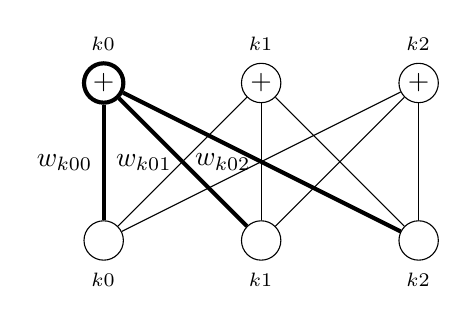
\begin{tikzpicture}[node distance=2cm, auto]

		% Upper layer nodes with increased size
		\node[draw, circle, minimum size=0.5cm,inner sep=1pt, line width=1.5pt] (A1) at (0, 2) {$+$};
		\node[draw, circle, minimum size=0.5cm,inner sep=1pt] (A2) at (2, 2) {$+$};
		\node[draw, circle, minimum size=0.5cm,inner sep=1pt] (A3) at (4, 2) {$+$};
		% Lower layer nodes with increase size
		\node[draw, circle, minimum size=0.5cm] (B1) at (0, 0) {};
		\node[draw, circle, minimum size=0.5cm] (B2) at (2, 0) {};
		\node[draw, circle, minimum size=0.5cm] (B3) at (4, 0) {};

		% Labels for the upper layer
		\node at (0, 2.5) {$\Qcircuit_{k0}$};
		\node at (2, 2.5) {$\Qcircuit_{k1}$};
		\node at (4, 2.5) {$\Qcircuit_{k2}$};

		% Labels for the lower layer
		\node at (0, -0.5) {$\tildeQcircuit_{k0}$};
		\node at (2, -0.5) {$\tildeQcircuit_{k1}$};
		\node at (4, -0.5) {$\tildeQcircuit_{k2}$};

		% Connecting upper layer to lower layer
		\foreach \i in {1,2,3}{
				\foreach \j in {1,2,3}{
						\draw (A\i) -- (B\j);
					}
			}



		% Thicker edges connected to the upper-left node
		\draw[line width=1.5pt] (A1) -- (B1) node[midway, left]{$w_{k00}$};
		\draw[line width=1.5pt] (A1) -- (B2) node[midway, left] {$w_{k01}$};
		\draw[line width=1.5pt] (A1) -- (B3) node[midway, left] {$w_{k02}$};

	\end{tikzpicture}
}
	\caption{
	Graphical representation of operator mixing as described in Equation~\ref{eq:operatormix}. The operators $\Qcircuit_{k0}$, $\Qcircuit_{k1}$, and $\Qcircuit_{k2}$ are all PSD matrices and constructed using the operators  $\tildeQcircuit_{k0}$, $\tildeQcircuit_{k1}$, and $\tildeQcircuit_{k2}$ using weighted sums. For $\Qcircuit_{k0}$ we also indicate the mixing weights $w_{k00}$, $w_{k01}$, and $w_{k02}$, which are positive real-valued scalars and satisfy $w_{k00}+ w_{k01}+w_{k02}=1$.
	}
	\label{fig:operatormixture}
\end{figure}






Recursively nesting such weighted sums of operators allows for representing a polynomial with exponentially many terms~\citep{martens2014expressive}.
However, in practice we only need to materialize these mixtures when computing $\sum_{\xvars \in \Omega(\Xvars) \pi_\Xvars(\xvars)}$ in order to normalize the probabilities.
If we evaluate a \noisepunc it suffices to evaluate the soft counting circuit $\qcircuit(\xvars)$ and the \punc $\punccircuit(\xvars)$ separately, and use the individual circuit evaluations to compute the unnormalized but bounded probability.

\citet{loconte2024relationship} proposed a similar combination of monotone and non-monotone circuits. This was motivated by their observation that the expressive power of monotone and squared circuits (a special case of positive operator circuits) are incomparable \citep{decolnet2021compilation}. That is, each of these circuit classes can express circuits that would lead to an exponential blow-up in the respective other circuit class.
Interestingly, we arrived at a similar construction by starting from noise in quantum circuits.























\section{Parametrizing \puncs}

In order to parametrize positive unitary circuits, we need to find a functional form of the bilinear forms such that Equation~\ref{def:eq:bilinear_psd} and Equation~\ref{def:eq:bilinear_unitpreserving} hold, and such that we have $A_k A_k^*=\mathbb{1}$.
For the latter we simply pick $A_k$ to be the (possibly truncated) orthonormal discrete Fourier transform matrix. This means that the $A_k$ are identical for all the leaves and that the leaves are parameter free but guarantees that we indeed have $A_kA_k^*?\mathbb{1}$.

For the bilinear forms we take inspiration from the probabilistic circuit literature and use a canonical polyadic ansatz~\citep{carroll1970analysis}.
\begin{align}
	\bilinear_k (\Ocircuit_{k_l}, \Ocircuit_{k_l} )
	=
	L_k \Ocircuit_{k_l} L_k^* \odot R_k \Ocircuit_{k_r} R_k^*,
	\label{eq:polyadicbilinear}
\end{align}
where $L_k$ and $R_k$ are complex valued matrices satisfying $L_k L_k^* \odot R_k  R_k^* = \mathbb{1}_{B\times B}$.

Assuming $O_{k_l}$ and $O_{k_r}$ are PSD we also have that $L_k \Ocircuit_{k_l} L_k^*$ and $R_k \Ocircuit_{k_r} R_k^*$ are PSD. Furthermore, using Schur's product theorem~\citep[p. 14, Theorem VII]{schur1911bemerkungen} that states that the Hadamard product of two PSD matrices is again PSD lets us conclude that parametrizing operator circuits with bilinear forms from Equation~\ref{eq:polyadicbilinear} results in the circuit being positive. For a discussion on the constraint $L_k L_k^* \odot R_k  R_k^* = \mathbb{1}_{B\times B}$ we point to Section~\ref{sec:efficient_param}.



\begin{restatable}{proposition}{propcomputationalcomplexity}
	\label{prop:computationalcomplexity}
	Let $\numvar$ be the number of variables $\xvars_k$,  having all the  domain size $\samplespacesize$, and let the $L_k$ and $R_k$ matrices be $\numbond\times \numbond$ square matrices, with $\numbond\leq \samplespacesize$.
	We can perform marginal inference in \puncs in $\bigO(\numvar \samplespacesize^3)$ when using the bilinear form from Equation~\ref{eq:polyadicbilinear}.
\end{restatable}

\begin{proof}
	See Append \ref{sec:proof:prop:computationalcomplexity}
\end{proof}












\subsection{The Vector Representation}
\label{sec:vpoc}

The matrix-matrix multiplication present in Equation~\ref{eq:polyadicbilinear} lead to the cubic computation cost per computation unit $\bigO (\samplespacesize^3)$ (\cf Section~\ref{sec:proof:prop:computationalcomplexity}). By exploiting the particular structure of the bilinear form in Equation~\ref{eq:polyadicbilinear} and by rearranging the operations performed in the operator circuit, we can avoid these matrix-matrix multiplications entirely and obtain matrix-vector multiplications instead. We call this alternative representation the \textit{vector} representation of an operator circuit.

\begin{definition}[Vector Representation]
	\label{def:vpoc}
	Let   $\xvars{=}\{\xvar_0,\dots ,\xvar_{\numvar{-}1}  \}$ be a set of $\numvar$ categorical variables with domains of size $\samplespacesize$.
	We define the vector representation of an operator circuit as a partition circuit whose computation units take the following functional form:
	\begin{align}
		{\vcircuit}_k(\xvars_k){=}
		\begin{cases}
			A_{k} \times  e_{\xvar_k},
			 & \text{if $k$ leaf}
			\\
			L_k {\times}  \vcircuit_{k_l} (\xvars_k)  \odot R_k {\times}  \vcircuit_{k_r} (\xvars_k),
			 & \text{else}
		\end{cases}
		\label{eq:vector_units}
	\end{align}
\end{definition}





\begin{restatable}{proposition}{propvoequiprob}
	\label{prop:voequiprob}
	The expression $\lVert \gamma \times \vcircuit_{\text{root}}(\xvars)\rVert^2$, with $\rho = \gamma \times \gamma^*$ computes the same probability as $\Tr [\Ocircuit_{\text{root}}(\xvars) \rho]$.
\end{restatable}

\begin{proof}
	See Section~\ref{sec:proof:prop:voequiprob}
\end{proof}

\begin{restatable}{proposition}{propcomputationalcomplexityvec}
	\label{prop:computationalcomplexityvec}
	\puncs in their vector representation compute joint probabilities in time $\bigO(\numvar \samplespacesize^2)$
\end{restatable}

\begin{proof}
	See Section~\ref{sec:proof:prop:computationalcomplexityvec}
\end{proof}

Note that the vector representation can only be used for computing joint probabilities as marginalizing out variables forces us to go to the matrix representation of operator circuits. Note also that the vector representation of \puncs can be seen as a PSD circuits~\cite{sladek2023encoding} or equivalently sum of squares circuits~\citep{loconte2024sum}, which we obtained by imposing a specific functional structure on the bilinear forms.

Having an efficient evaluation for \puncs in their vector representation also means that we can evaluate \noisepuncs more efficiently as we can compute $\qcircuit_{root}(\xvars)$ and $\pi_\Xvars(\xvars)$ separately, with the former having a computational complexity of $\bigO(\numvar \numcomponents \samplespacesize + \numvar \numcomponents^2)$.
Computing the normalization constant for a \noisepunc is more involved, and we discuss it along with its computational complexity in Appendix~\ref{sec:noisepuncnormalization}. However, we note that it is still feasible in polytime.




%%%%%%%%%%%%%%%%%%%%%%%%%%%%%%%%%%%%%%%%%%%%%%%%%%%%%%%%%%%%%%%%%%%%%%%%%%%%%%%%%
%%%%%%%%%%%%%%%%%%%%%%%%%%%%%%%%%%%%%%%%%%%%%%%%%%%%%%%%%%%%%%%%%%%%%%%%%%%%%%%%%
%%%%%%%%%%%%%%%%%%%%%%%%%%%%%%%%%%%%%%%%%%%%%%%%%%%%%%%%%%%%%%%%%%%%%%%%%%%%
















\subsection{An Efficient Parametrization}
\label{sec:efficient_param}

Having specified the functional form of the positive unitary circuits using polyadic bilinear forms we would also like to find an efficient parametrization of the $\gamma$, $L_k$, and $R_k$ matrices that is amenable to unconstrained gradient descent optimization. For $\gamma$ this is rather straightforward as we can simply use:
$
	\gamma = \frac{\tilde{\gamma}}{\sqrt{\Tr [\tilde{\gamma} \tilde{\gamma}^*]}},
$
where $\tilde{\gamma}\in \mathbb{C}^{B\times B}$ is an arbitrary complex values matrix. Note that we have almost by definition $\Tr [\rho] = 1$.

% Efficiently parametrizing the bilinear form such that they are amenable to unconstrained gradient based optimization is a bit more intricate. We refer the reader to Appendix~\ref{sec:bilinearparametrization}. The main idea is to use products of diagonal and circulant matrices~\citep{araujo2020understanding}, which can be parametrized using discrete Fourier transform matrices.


For the $L_k$ and $R_k$ matrices we make some further specifying choices. Consider the real-valued diagonal matrix $D_k \in \mathbb{R^{B\times B}}$ and the two unitary matrices $U_k \in \mathbb{C^{B\times B}}$ and $V_k \in \mathbb{C^{B\times B}}$, which we use to construct the $L_k$ and $R_k$ matrices:
\begin{align}
	L_k  = D_k^{\nicefrac{1}{2}} U_k,
	\quad \text{and} \quad
	R_k  = D_k^{-\nicefrac{1}{2}} V_k.
\end{align}


We can verify that this parametrization satisfies the unit preserving condition of for the bilinear form (\cf Definition~\ref{def:bilinear_unitpreserving}).
\begin{align}
	B_k(\mathbb{1}_{B\times B}, \mathbb{1}_{B\times B})
	 & = L_k \mathbb{1}_{B\times B} L_k^* \odot R_k \mathbb{1}_{B\times B} R_k^*
	\nonumber
	% \\
	%  & = L_k L_k^* \odot R_k R_k^*
	% \nonumber
	\\
	 & =D_k^{\nicefrac{1}{2}} U_k  U_k^* D_k^{\nicefrac{1}{2}}
	{\odot}
	D_k^{-\nicefrac{1}{2}} V_k  V_k^* D_k^{-\nicefrac{1}{2}}
	\nonumber
	\\
	%  & =D_k \odot D_k^{-1}
	% \nonumber
	% \\
	 & = \mathbb{1}_{B\times B}
\end{align}
While we now have a prescription to parametrize \puncs, one problem remains: unitary matrices are notoriously difficult to parametrize efficiently~\citep{kiani2022projunn,jing2017tunable,lezcano2019cheap,mhammedi2017efficient,wisdom2016full}.

We will take a practical approach here and parametrize the unitary matrices using a product of a diagonal and circulant matrix:
\begin{align}
	U_k = \Lambda_{U_k} F_B \Sigma_{U_k} F_B^{*}
	\quad \text{and} \quad
	V_k = \Lambda_{V_k} F_B \Sigma_{V_k} F_B^{*}.
\end{align}
Here $\Lambda_{U_k}$, $\Lambda_{V_k}$,  $\Sigma_{U_k}$, and $\Sigma_{V_k}$ are diagonal matrices whose entries have no magnitude, \ie they are of the form $e^{i\phi}$ with $\phi \in \mathbb{R}$. Furthermore, $F_B$ denotes the orthonormalized B-point discrete Fourier transform matrix, and we exploit the fact any circulant $B\times B$ matrix can be written as a diagonal matrix sandwidched between $F_B$ and $F_B^*$. Recalling that $F_B$ is unitary it is again straightforward to show that this parametrization yields unitary matrices. We also refer the interested reader to ~\citet{araujo2020understanding} for a in depth discussion of diagonal-circulant parametrization of neural networks.

While using this diagonal-circulant parametrization does not cover the entire space of unitary matrices it has the advantage of being parametrizable with unconstrained parameters. Furthermore, using the fact that mulitplying a discrete Fourier transform matrix with a vector can be done on $\bigO(\numbond \log \numbond)$ brings down the computational cost of computing the bilinear form from $\bigO(\numbond^2)$.














Lastly,  for the set of  basis vectors $\{e_{\xvar_s} \}_{s=0}^{\samplespacesize-1}$ in the leaves we choose the set of standard basis vectors, \ie one-hot unit vectors, with each basis vector $e_s$ corresponding to a random outcome. Although different choices of basis vectors would be valid as well, For the $A_k$ we use, as already mentioned, the orthonormal discrete Fourier transform matrix, which we truncate if $\numbond<\samplespacesize$.







%%%%%%%%%%%%%%%%%%%%%%%%%%%%%%%%%%%%%%%%%%%%%%%%%%%%%%%%%%%%%%%%%%%%%%%%%%%%%%%%%
%%%%%%%%%%%%%%%%%%%%%%%%%%%%%%%%%%%%%%%%%%%%%%%%%%%%%%%%%%%%%%%%%%%%%%%%%%%%%%%%%
%%%%%%%%%%%%%%%%%%%%%%%%%%%%%%%%%%%%%%%%%%%%%%%%%%%%%%%%%%%%%%%%%%%%%%%%%%%%


\section{Related Work}
\label{sec:related}


\subsection{Squared Cirucuits}

The work closest related to ours are the \text{sum of compatible square circuits} by \citet{loconte2024sum}.
As shown in Section~\ref{sec:vpoc} we recover sum of square circuits (introduced earlier as PSD circuits by \citet{sladek2023encoding}) if we use a polyadic decomposition in the bilinear form, \cf Equation~\ref{eq:polyadicbilinear}.
A non-polyadic decomposition would have resulted in a computation graph closer to that of \textit{inception circuits} introduced by \citet{wangrelationship}. Such a choice, however, increases the computation cost per unit in the partition circuit from quadratic (using the vector representation) to cubic (using the operator representation).

Our positive unit preserving operator circuits provide also a different perspective on constructing non-monotone circuits. While the methods described in ~\citep{sladek2023encoding,loconte2024subtractive,loconte2024sum,wangrelationship} regard such circuits as sum of squares, we interpret them as probabilistic events described by positive semidefinite matrices that are combined within a circuit using unit preserving bilinear forms. As such, we also establish a strong link between the circuit literature and quantum information theory.

From a practical perspective, the (sub-complete) distributions encoded with \puncs and \noisepuncs tackle one of the main shortcoming of sum of squares type circuits: we do not need to compute a normalization constant to ensure that event probabilities are bounded. This especially useful during training, as it means that updating the parameters of the model still guarantees the event probability to be bounded. Otherwise one would have to compute a normalization constant and differentiate through it at every iteration of the parameter updates. This potentially hinder scaling up non-monotone models as computing the normalization constant cannot be done in the vector representation (quadratic cost) but requires matrix-matrix multiplications with cubic cost. For \puncs computing this normalization is not necessary at all and for \noisepunc we only need to compute the normalization constant once training has finished as post-processing step.

\subsection{Tensor Networks}

As already pointed out by \citet{loconte2024subtractive,loconte2024sum} squared circuits and monotone circuits share many similarities with \textit{tensor networks}~\citep{orus2014practical,white1992density}
developed in the condensed matter physics community and have in recent years also been applied to tackle problems in supervised as well as unsupervised machine learning~\citep{cheng2019tree,han2018unsupervised,stoudenmire2016supervised}. In this regard and given that tensor networks originate in the physics community, it is rather surprising that tensor networks have so far, and to the best of our knowledge, not been formulated using POVMs.

Using our POVM formulation for \puncs is, however, not only theoretically elegant but has also practical benefits: using this formalism leads to circuits that are normalized by construction, and we can perform learning simply by optimizing the likelihood. We contrast this to the sweeping algorithms that are usually deployed in the tensor network literature, where blocks of variables are optimized one at the time while the remaining variables are held constant. It appears that this approach is inspired by the variational ansatz taken in the density-matrix renormalization group algorithm~\citep{white1992density}, which is the original algorithm for tensor networks.
Alternatives to this sweeping approach have also been proposed, such as an intricate Riemannian gradient descent optimization scheme that conserves unitarity of matrices, but are rather costly to run.

We would also like to point out a theoretical result from the tensor network literature stating that picking a complex-valued parametrization instead of a real-valued one can lead to an arbitrarily large reduction in the number of parameters~\citep{glasser2019expressive}. While this result is formulated with respect to (exact) low rank tensor decomposition and does not apply directly to the problem of learning parameters via gradient descent, we consider this observation to be a strong theoretical indicator for the superiority of complex numbers over real numbers when parametrizing probabilistic circuits. A similar argument has also been made by \citet{gao2022enhancing} in the context of hidden Markov models.

\subsection{Theoretical Studies}

First theoretical results on expressive power of polynomial functions, \ie circuits and tensor networks, were presented in the tensor network literature in the context of tensor decomposition \citep{glasser2019expressive} and complex-valued hidden Markov models \citep{gao2022enhancing}. Recently, the works of \citet{loconte2024subtractive,loconte2024sum} and \citet{wangrelationship} have studied the relationship of different circuits classes more carefully, as well. Additionally, \citet{loconte2024sum} pointed out links between tensor networks and the circuit literature and were able to generalize earlier results from the tensor network literature by~\citet{glasser2019expressive}.

Finally, we would also like to point out theoretical results n the statistical relational AI literature. Specifically, \citet{buchman2017rules}, and \citet{kuzelka2020complex} noted that using only real-valued parametrizations (including negatives~\citep{buchman2017negative}), \ie monotone functions exclusively, does not allow for fully expressive models.



































\section{Experimental Evaluation}
\label{sec:experiments}


\textbf{Experimental Setup}


For our experimental evaluation we used the MNIST family of datasets. That is, the original MNIST~\citep{deng2012mnist}, FashionMNIST~\citep{xiao2017fashion}, and also EMNIST~\citep{cohen2017emnist}.
For the implementation we used PyTorch together with the Einops library~\citep{rogozhnikov2022einops}. We set up our experiments in Lightning\footnote{\url{https://lightning.ai/}} and ran them on a DGX-2 machine with V100 Nvidia cards.

We compare different methods using the \textit{bits per dimension} metric, which is calculated from the average negative log-likelihood ($\overline{NLL}$) as follows: $bpd {=} \nicefrac{\overline{NLL}}{(\log{2} \times D)}$ ($D{=}28^2$ for MNIST datasets).



\textbf{Training Positive Operator Circuits}

In our experiments we estimate the density of the different MNIST datasets by maximizing a parametrized likelihood function. We construct this  function using a positive vector circuit.
In order to build the underlying partition circuit,
we follow the approach described by \citet{zuidberg2024probabilistic}: we start with a grid of $28\times 28$ pixels and merge, in an alternating fashion, rows and columns of the image.
We also allow for merging three partitions into  a single partition, thereby breaking the binary character of the partition trees used so far.
Having three instead of two partitions being merged can easily be accommodated for by using a Hadamard product with three factors instead of two in the internal units of a \pvc. Ultimately, this allows us to handle layers with an uneven number of partitions.
At the leaves we encode pixel values by associating each value to one of $256$ standard basis vector of $\mathbb{R}^{256}$.

We performed training by minimizing the negative log-likelihood using Adam~\citep{kingma2014adam} with default hyperparameters, batch size of $50$, over $100$ epochs.
The best model was selected using a $90-10$ train-validation data split where we monitored the negative log-likelihood on the validation set.
We did not perform any hyperparameter search.
Further details can be found in the configuration files of the experiments.



\textbf{State-of-the-Art Baselines}

We compare \pvcs to three state-of-the-art tractable density estimators from the literature: quadrature of probabilistic circuits (QPCs)~\citep{gala2024probabilistic}, hidden Chow-Liu trees (HCLTs)~\citep{liu2021tractable}, and sparse HCLTs (SHCLTs)~\citep{dang2022sparse}.
All three methods are probabilistic circuits and they all use hidden Chow-Liu trees as their underlying structure. This tree is learned and dataset specific. The difference between QPCs and HCLTs is that the former is obtained by approximating a continuous latent variable extension of probabilistic circuits using numerical quadrature. The difference between HCLTs and SHCLTs is that the latter allows for dynamically adapting the number of components per partition during parameter learning. This means that SHCLTs can focus their computational budget on information-rich parts of the circuit.



\textbf{Q1: How Do the Different \pvc Parametrizations Fair Against Each Other?}

We construct \pvcs following the prescription of \cite{zuidberg2024probabilistic}, as described above. Furthermore, we use $B=128$ components per partition.
As for the parametrization we study four different variants:
$\mathrm{PVX}_{0}^{FR}$,
$\mathrm{PVX}_{2\pi}^{FR}$,
$\mathrm{PVX}_{0}^{R1}$, and
$\mathrm{PVX}_{2\pi}^{R1}$.
The subscripts ($0$ or $2\pi$) indicate whether we limit the phase to be zero or whether we allow the phase to be a learnable parameter. Note that having a tunable phase doubles the number of (real-valued) parameters. The superscript indicates whether the parametrization uses a full-rank ($FR$) density matrix in the root or a rank-one ($R1$) density matrix.
As such, $\mathrm{PVX}_{0}^{R1}$ is equivalent to the  squared monotonic probabilistic circuits (\smpcs) used in ~\cite{loconte2024subtractive}, and $\mathrm{PVX}_{2\pi}^{R1}$ generalizes their \snpcs from the real domain to the entire complex domain. Concretely, \smpcs are rank-one \pvcs with the phase fixed to zero and \snpcs are rank-one \pvcs with the phase fixed to values in the set $\{0, \pi \}$. We do not experiment on the latter.

We report the obtained bpds for the different \pvc parametrizations in the first four columns of Table~\ref{tab:mnist}. In general, we see that the complex-valued parametrizations are either on par or outperform the corresponding zero-phase parametrizations.
The notable exception is the FashionMNIST benchmark where the two parametrizations with no phase ($\mathrm{PVX}_{0}^{FR}$ and $\mathrm{PVX}_{0}^{R1}$) perform best.
Comparing full-rank to rank-one parametrizations we see a more important impact for the zero-phase parametrization than for the complex-valued parametrization.


Overall, $\mathrm{PVX}_{2\pi}^{FR}$ constitutes the best performing parametrization being best-in-class on all benchmarks but FashionMNIST.


\begin{table*}[t]
\centering
\caption{Test set bpd for MNIST datasets (lower is better).}
 \label{tab:mnist}
\begin{tabular}{lccccccc}
 & $\mathrm{PVX}_{0}^{FR}$ & $\mathrm{PVX}_{2\pi}^{FR}$ & $\mathrm{PVX}_{0}^{R1}$ & $\mathrm{PVX}_{2\pi}^{R1}$ & QPC & HCLT & SHCLT \\

\cmidrule(lr)
{2-5}\cmidrule(lr){6-8}
MNIST & $1.16$ & $1.16$ & $1.24$ & $1.17$ & $1.18$ & $1.21$ & $1.14$ \\
FashionMNIST & $3.37$ & $3.55$ & $3.44$ & $3.55$ & $3.27$ & $3.34$ & $3.27$ \\
E-MNIST & $1.69$ & $1.63$ & $1.76$ & $1.64$ & $1.66$ & $1.70$ & $1.52$ \\
E-LETTERS & $1.62$ & $1.60$ & $1.70$ & $1.61$ & $1.70$ & $1.75$ & $1.58$ \\
E-BALANCED & $1.65$ & $1.64$ & $1.73$ & $1.64$ & $1.73$ & $1.78$ & $1.60$ \\
E-BYCLASS & $1.47$ & $1.47$ & $1.56$ & $1.49$ & $1.67$ & $1.73$ & $1.54$ \\
\end{tabular}
\end{table*}









\textbf{Q2: How Do \pvcs Fair Against the State of the Art?}

In order to compare \pvcs to state-of-the-art circuits all methods (\pvc, QPC, HCLT, SHCLT) were given a computational budget of $B=128$ components per partition (on average for SHCLT).
The results for the competing methods were taken from the respective papers -- except for HCLTs. For HCLTs we took the bpds reported by \citet{gala2024probabilistic} as they achieved stronger results with their implementation compared to the originally reported performance~\citep{liu2021tractable}.

We see in Table~\ref{tab:mnist} that QPCs and HCLTs are in general outperformed by \pvc -- in particular $\mathrm{PVX}_{2\pi}^{FR}$. The FashionMNIST benchmark constitutes again an outlier in this regard.
The only methods outperforming \pvcs are the SHCLTs, which is due to them being able to dynamically allocate compute budget to informative parts of the circuit.
It is noteworthy that for the EMNIST-BYCLASS benchmark all four  \pvc parametrization exhibit strong performance with  $\mathrm{PVX}_{2\pi}^{FR}$ and $\mathrm{PVX}_{2\pi}^{R1}$ even outcompeting SHCLTs.


\textbf{Discussion}

In our experimental evaluation we did not perform an explicit comparison to the method of \citet{loconte2024subtractive} as they were not able to find any improvements of allowing non-negative parameters in probabilistic circuit for discrete data. They stipulated that
\say{simple categorical distribution can already capture any discrete distribution with finite support and a (subtractive) mixture thereof might not yield additional benefits}.
In our experimental evaluation we refute this conjecture, and show that using complex-valued parameters leads to noticeable gains when performing density estimation on discrete data.
The exception being of course the FashionMNIST benchmark. We believe that this is due to our optimization method that was not tuned in any way.
In this regard we believe that developing tailor-made optimization algorithms for \pvcs might further boost their performance.
Furthermore, one can envisage, similar to SHCLTs, dynamically adapting the compute budget per partition, which should again improve the density estimation capacities of \pvcs.






\section{Conclusions \& Future Work}
\label{sec:conclusions}

Based on first principles from quantum information theory, we constructed positive operator circuits -- a novel class of probabilistic tractable models:
Their construction as partition circuits allows for layer-wise parallelization and execution on modern machine learning hardware.
Using unconstrained gradient-descent we showed that \pocs, and \pvcs specifically, constitute a promising addition to the zoo of tractable probabilistic models.

In future work we would like to investigate in more detail theoretical properties of \pocs and how they differ from other tractable models. Ideally one would find an exponential separation between real-valued and complex-valued circuits. On the practical side it remains, however, to be seen whether such a separation has an equally important impact on real-world datasets.

This relates to another open question,  that of learning in \pocs. We presented a rather simple learning approach for parameters tailored towards neural architecture. It might be the case that more sophisticated techniques have to be deployed for large-scale \pocs, as they might exhibit the problem of barren plateaus~\citep{ragone2023unified} -- a well known issue in quantum machine learning~\citep{biamonte2017quantum,huggins2019towards}.
Furthermore, and as already pointed out by~\citet{loconte2024subtractive}, computing the normalization constant $Z$ requires the evaluation of the circuit in the \poc representation. This gives rise to a rather expensive cubic computation cost during learning (when compared to the quadratic cost of \pvc evaluations). Avoiding this issue would allow to drastically scale \pvcs. In order, to scale \pvcs it might also be necessary to use more sophisticated structures than binary trees with every partition having the same number of components $B$ per partition, \cf SHCLTs.



















